\documentclass{article}
\usepackage{bigstrut}
\usepackage{adjustbox}
\usepackage{graphicx}^^M
\graphicspath{ {images/} }
\usepackage[T1]{fontenc}
\usepackage{float}

\usepackage[english]{babel}
\usepackage[utf8]{inputenc}
\usepackage{indentfirst}

\addtolength{\oddsidemargin}{-.875in}
\addtolength{\evensidemargin}{-.875in}
\addtolength{\textwidth}{1.75in}
\addtolength{\textheight}{1in}

\begin{document}
\title{}
\begin{titlepage}
    \centering
	{\scshape\LARGE Lab 2: Corrosion and Electrodeposition\par}
	\vspace{1cm}
	{\scshape Aristide Muscariello Jr.: Manager,Technician \hfill ID\#:10406472 \par}
	{\scshape Marcin Wisniowski: Technician,Recorder \hfill ID\#:10417225\par}
	\vfill
	{\scshape Design V, Week 2\par}
	\vspace{.5cm}
	{\scshape Laboratory Performed: January 30th, 2018\\Stevens Institute of Technology\\E-231 Section I Group 2\par}
	\vspace{.5cm}
	{\scshape supervised by\\Mr. Di Wu, Mr. Kai Zong \par}
    \vfill
% Bottom of the page
	{\scshape“I pledge my honor that I have abided by the Stevens Honor System.”\par}
	\vspace{.5cm}
	{\scshape Aristide Muscariello Jr. \hfill Date: 02/1/18\\Marcin Wisniowski \hfill Date: 02/1/18\\}
	\vspace{3cm}
\end{titlepage}

\section{Introduction}
This lab looks to explore the effects of oxidation when iron is exposed to the elements and finding a way to limit its negative effects. Corrosion refers to the degradation of a material, typically a metal or alloy, due to an electrochemical reaction with its environment. The most notable effect of corrosion, and most widely popularized is rust, the effect of oxidation onto iron. While iron is found in nature as an oxide, it is only useful to use in society after refining into the metal that we know. After refining, however the iron will convert back to an oxide if exposed to the proper conditions. This is a negative reaction to the human population, as this weaker rust is less useful in the construction industry. It is therefore important to learn how to prevent corrosion in order to keep iron tools or materials from becoming ineffective over time. 

\subsection{Objective}
Over the course of this lab, the group looks to learn to:
\begin{enumerate}
	\item Define corrosion and identify at least five engineering applications in which corrosion plays a significant role in materials selection and design. 
	\item Conduct and characterize a coating process using electrodeposition. 
	\item Characterize the corrosion behavior and corrosion products of steel and galvanized steel in some typical application environments. 
	\item Critique the advantages and disadvantages of common corrosion protection approaches.
\end{enumerate}

\subsection{Procedure}
The lab was split into three separate experiments to explore the effects of rust and how to distinguish it. The group was able to observe the different effects corrosion has on tools over time, distinguish differing rates of corrosion in various environmental solutions and learn to create an electrochemical cell in order to allow the deposition of zinc onto a steel plate in order to protect it from the effects of corrosion.   

\subsubsection{Electrochemical Cell}
The group first decided to create an electrochemical cell to have electrodeposition of zinc onto a steel plate. This experiment had to sit idle for 10 minutes while the ionization took place, so it was effective to begin it first and do the other experiments in the waiting portion of this experiment.

\begin{figure}[ht]
\caption{Electroplating}
\centering
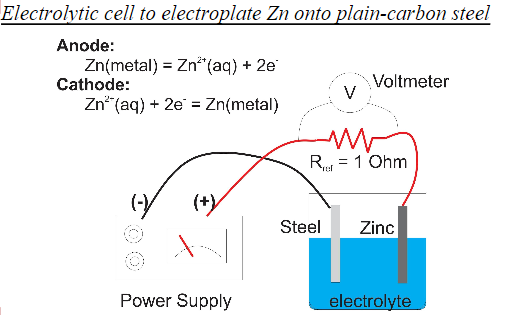
\includegraphics[width=200pt]{Electroplating.png}
\end{figure}

To start, the group obtained samples of both zinc and steel and sanded them down to be clean for testing. Then, the dimensions for both metals were recorded for future calculations. The group also needed to test the resistance of power supply in order to achieve a current between 0.5-1.0 amps. The electrochemical cell was constructed and left to sit idle for 10 minutes at the appropriate amperage for the reaction to take place. After the deposition concluded, the zinc and steel samples were weighed again for calculations.

The group expected that the zinc would lose weight in equal quantity to the weight that the steel would gain, due to the chemical reaction moving zinc onto the surface of the steel plate. 

\subsubsection{Corrosion of Steel and Electroplated Steel}
While waiting for the electrodeposition to conclude, the group observed prepared solutions containing either zinc-galvanized roofing nails or an uncoated steel sample to see the corrosive effects different solutions of liquids had on the materials.

\subsubsection{Observation of Corrosion Products}
Similarly, While waiting for the electrodeposition to conclude, the group observed the physical characteristics of rust on steel tools that were exposed to moisture in the real world.

\section{Results}
\subsection{Experiment 1: Electrochemical Cell}
Ultimately, the electrochemical cell ended up removing atoms from the zinc plate and moving them over to the steel plate through the chemical reaction, as was predicted. This could mostly be seen in the physical appearance of the now galvanized steel plate as well as the new weights that were recorded after the reaction took place, showing that the zinc plate had lost weight at the same time that the steel plate gained weight. Furthermore, the total weight of both plates stayed the same, showing that at least to the accuracy of the scale used, no zinc or steel was lost in the process of the reaction. 

{\renewcommand{\arraystretch}{1.2}
\begin{table}[H]
\begin{center}
\begin{tabular}{c|c|c|c|c|c}
Material & Width & Length & Thickness & Weight(before) & Weight(after)\\
\hline
Zinc & 25mm & 47.9mm & 1.06mm & 11.15g & 10.85g\\
Steel & 24.5mm & 49.7mm & 1.30mm & 13.0 g & 13.35g\\
\end{tabular}
\caption{Physical Properties of Zinc and Steel}
\end{center}
\end{table}

Theoretically, this chemical reaction can be displayed as: 
$$Zn^{2+} + 2e^- = Zn$$
In this chemical reaction. Multiple zinc atoms were deposited from the Zn plate onto the Steel plate. In order to calculate the theoretical amount, we use the equation:

$$Q = I*t = 600 A s$$
$$Ne^- = \frac{I*t}{1e^-} = \frac{600 A s}{1.6 x 10^{-19} C} = 3.75 x 10^{21}$$
$$N_{Zn} = \frac{1}{2}Ne^- = 1.875 x 10^{21}$$
$$M_{Zn} = \frac{65.38g}{mol} ; \rho_{Zn} = \frac{7.14g}{cm^3} ; N_A = \frac{6.02 x 10^{23}}{mol}$$
$$\Delta Mass = \frac{\phi M_{Zn}}{2eN_A} = N_{Zn} \frac{M_{Zn}}{N_A} = 1.875 x 10^{21} * \frac{65.385 g}{mol} * \frac{mol}{6.02 x 10^{23}} = 0.2036 g$$
$$\Delta Thickness = \frac{\Delta V}{l * w} = \frac{\Delta Mass}{l*w* \rho_{Zn}} = \frac{0.2036 g}{630.1 x 10^{-2} cm^2 * 7.14 g/cm^3} = 4.525 x 10^{-3}cm = 4.525 x 10^{-2} mm$$

Comparing the theoretical weight change with the measured amount of weight change of Zinc, the group saw that theoretically after 10 minutes, the group would have seen the Steel gain 0.2036 grams. In the actual testing environment, the steel changed from a weight of 13.0 grams to a weight of 13.35g, making the $\Delta Mass = 0.35g$. In real testing, this shows that more zinc was deposited than expected. This may have been due to a higher amperage or longer testing time.

\begin{figure}[ht]
\caption{Zinc Deposit on Steel Plate}
\centering
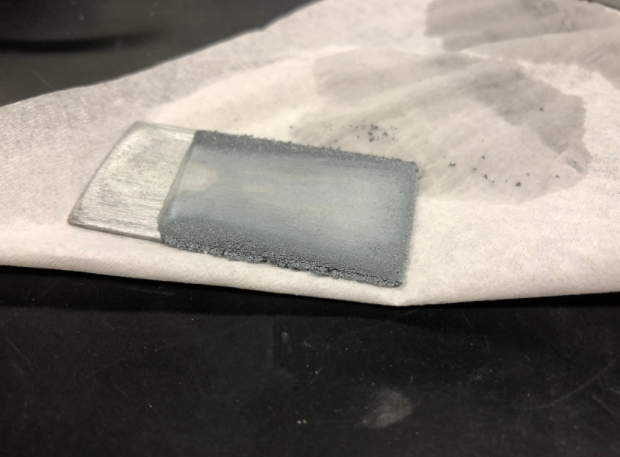
\includegraphics[width=300pt]{ZincDeposition.png}
\end{figure}

\subsection{Experiment 2: Corrosion of Steel and Galvanized Steel}
	This experiment was more of a demonstration to the lab group of how zinc coated and non-zinc coated materials react to different environments. The team hypothesized that the materials that were given a zinc coating would be more resistant to the effects of corrosion while the non-treated materials would have been eroded quite badly. 
    
\begin{figure}[ht]
\caption{Beakers of Steel Plates}
\centering
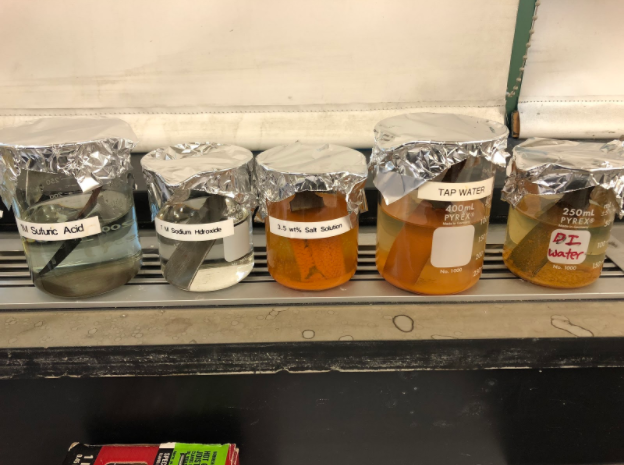
\includegraphics[width=250pt]{Beakers1.png}
\end{figure}

\begin{figure}[ht]
\caption{Beakers of Galvanized Roofing Nails}
\centering
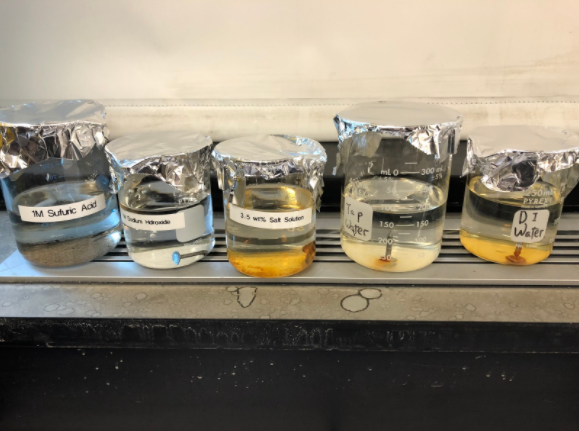
\includegraphics[width=250pt]{Beakers2.png}
\end{figure}
\newpage

The hypothesis wound up being backed up by what was observed: the treated materials fared much better than the bare materials in all the mixtures, with the exception of distilled water, which seemed to damage both pieces similarly.

\subsection{Experiment 3: Observation of Corroded Products}
	The final procedure had the lab team observe rusted hand tools. Sandpaper would be used to try and remove the rust on the tools to find if the rust was formed on the surface, or if it was on the inside of the tool. The team’s hypothesis was that the rust would be able to be removed with the sandpaper, but at the cost of losing some steel on which the rust had formed.
    
	When the team first examined the tools, they used only the provided latex gloves to try and remove the rust. It was unclear whether or not the rust was actually being removed from the tool or if the residue left on the gloves was just small residue that was lying on top of the steel. Still, there was a small amount of rust on the gloves, seen as an orange powder. 
    
	The team then used a small square of sandpaper to see if more rust could be removed. The rust was definitely being pulled from the surface of the tool much more effectively than with just the latex gloves. The team also noticed that after using the sandpaper, small streaks of shiny, fresh steel were visible below the outermost surface of the tool, suggesting that the original hypothesis had been accurate: a very small amount of the steel was being pulled off of the tool along with the rust layer that had formed. 
    
\begin{figure}[ht]
\caption{Rusted Hand Tool}
\centering
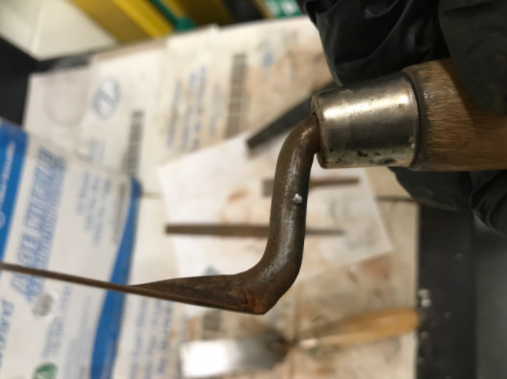
\includegraphics[width=300pt]{HandTools.png}
\end{figure}
    
	The team finished this portion of the experiment by wetting the tool they used to test their hypothesis. This would allow a new layer of rust to form for future lab groups to conduct tests.

\section{Discussion and Conclusions}
The group can conclude that electrodeposition is a valuable solution to the effects of rust and oxidation of metals like iron and steel. Initially, the group expected that galvanizing would have small effects on the physical protection of materials from rust. However, after looking at the coloration of steel plates in different solutions, the difference in rust exposure was drastically reduced. Similarly, the group was impressed with the thickness and amount of zinc that deposited onto the steel plate during the electrodeposition experiment. We initially hypothesized that the zinc would transfer over, but the coating was much thicker than expected. In the end, the group learned both how electrodeposition can be an effective way of minimizing rust formation, but also how it could be a costly solution both in materials and time. 

\section{Broader Impacts}
\begin{enumerate}
\item Identify and briefly describe one other engineering or manufacturing application of electrodeposition. 
\paragraph{}
Electroplating can be used to increase the toughness of a material, simply by adding a small “shell” to the outside of the treated component. Additionally, one can greatly reduce the rate of corrosion on a material by adding a protective layer of a more robust material. Perhaps a more practical use of electroplating is its ability to increase the tensile strength and hardness of the surface of a material. If a completed material is found to be too hard/too soft after application, engineers can use electroplating to coat the material in a softer shell thus eliminating the need to manufacture a whole new part. Cost is, of course, the main issue that comes up with electroplating as in some cases it may be too complicated to effectively treat a material.

\item Contrast the protection offered by coatings (such as paint)with that provided by galvanizing of steel samples. Include both advantages and disadvantages of each. 

\paragraph{}
The electroplating experiment demonstrated to the group how properties of a material can be altered to change how a component or any treated surface in general reacts to different environments. In a more basic case, a simple coating (i.e. paint) can be used to provide extra protection to the surface it is applied to. This solution is very cost effective and simple to apply, but provides minimum protection against potential weathering and corrosion.

\end{enumerate}



\end{document}